\documentclass[12pt]{article}\usepackage[]{graphicx}\usepackage[]{xcolor}
\usepackage{fullpage}
% maxwidth is the original width if it is less than linewidth
% otherwise use linewidth (to make sure the graphics do not exceed the margin)
\makeatletter
\def\maxwidth{ %
  \ifdim\Gin@nat@width>\linewidth
    \linewidth
  \else
    \Gin@nat@width
  \fi
}
\makeatother

\definecolor{fgcolor}{rgb}{0.345, 0.345, 0.345}
\newcommand{\hlnum}[1]{\textcolor[rgb]{0.686,0.059,0.569}{#1}}%
\newcommand{\hlstr}[1]{\textcolor[rgb]{0.192,0.494,0.8}{#1}}%
\newcommand{\hlcom}[1]{\textcolor[rgb]{0.678,0.584,0.686}{\textit{#1}}}%
\newcommand{\hlopt}[1]{\textcolor[rgb]{0,0,0}{#1}}%
\newcommand{\hlstd}[1]{\textcolor[rgb]{0.345,0.345,0.345}{#1}}%
\newcommand{\hlkwa}[1]{\textcolor[rgb]{0.161,0.373,0.58}{\textbf{#1}}}%
\newcommand{\hlkwb}[1]{\textcolor[rgb]{0.69,0.353,0.396}{#1}}%
\newcommand{\hlkwc}[1]{\textcolor[rgb]{0.333,0.667,0.333}{#1}}%
\newcommand{\hlkwd}[1]{\textcolor[rgb]{0.737,0.353,0.396}{\textbf{#1}}}%
\let\hlipl\hlkwb

\usepackage{framed}
\makeatletter
\newenvironment{kframe}{%
 \def\at@end@of@kframe{}%
 \ifinner\ifhmode%
  \def\at@end@of@kframe{\end{minipage}}%
  \begin{minipage}{\columnwidth}%
 \fi\fi%
 \def\FrameCommand##1{\hskip\@totalleftmargin \hskip-\fboxsep
 \colorbox{shadecolor}{##1}\hskip-\fboxsep
     % There is no \\@totalrightmargin, so:
     \hskip-\linewidth \hskip-\@totalleftmargin \hskip\columnwidth}%
 \MakeFramed {\advance\hsize-\width
   \@totalleftmargin\z@ \linewidth\hsize
   \@setminipage}}%
 {\par\unskip\endMakeFramed%
 \at@end@of@kframe}
\makeatother

\definecolor{shadecolor}{rgb}{.97, .97, .97}
\definecolor{messagecolor}{rgb}{0, 0, 0}
\definecolor{warningcolor}{rgb}{1, 0, 1}
\definecolor{errorcolor}{rgb}{1, 0, 0}
\newenvironment{knitrout}{}{} % an empty environment to be redefined in TeX

\usepackage{alltt}
%\usepackage{fullpage}
\usepackage{graphicx}
\usepackage[utf8]{inputenc}
\usepackage{amsmath}
\usepackage{graphics}
\usepackage{float}
\usepackage{xcolor}
\usepackage{geometry}
\usepackage[top=20pt,bottom=20pt,right=15pt,left=15pt]{geometry}
\usepackage{tikz}
\usetikzlibrary{shapes, arrows}
\usepackage[utf8]{inputenc}
\usepackage{amsmath}
\usepackage{graphics}
\usepackage{xcolor}
\usepackage{enumitem}
\usepackage{longtable}
\usepackage{array}
\numberwithin{equation}{section}
\numberwithin{figure}{section}
\newlist{bracketedromanenum}{enumerate}{1}
\setlist[bracketedromanenum]{
	label={(\roman*)},
	ref={\roman*},
	itemsep=0.5em,
	topsep=0.5em
}
\IfFileExists{upquote.sty}{\usepackage{upquote}}{}
\begin{document}
	\begin{titlepage}
		
		\begin{center}
			
			
\includegraphics[width=0.3\textwidth]{UoN_Logo.png}\\
			\vspace{0.3cm}
			UNIVERSITY OF NAIROBI\\
			FACULTY OF SCIENCE AND TECHNOLOGY\\
			DEPARTMENT OF MATHEMATICS\\
			\vspace{0.7cm}
			

	\textbf{Modeling Depression Severity among Caregivers in a Rural Setting using Ordinal Logistic Regression}
			
			\vspace{0.5cm}
			BY:\\
			
			BEVERLY KIND               : \hspace{0.2cm}    I63/4240/2019\\
			\vspace{0.5cm}
			WAMBUA CHARLES             : \hspace{0.2cm}    I63/4248/2019\\
			
			\vspace{0.5cm}
			ODHIAMBO KENNEDY           : \hspace{0.2cm}    I63/4282/2019\\
			\vspace{0.5cm}
			NYAENYA DOMINIC            : \hspace{0.2cm}    I63/4261/2019\\
			\vspace{0.5cm}
			PETER DOKTA               : \hspace{0.2cm}    I63/136668/2019\\
			\vspace{0.7cm}
			
			
			\vspace{0.7cm}
A project submitted to the Department of Mathematics in Partial Fulfillment for award of the Degree of Bachelor of Science in Statistics\\
			\vspace{0.5cm}
			JULY 2023
			
			
		\end{center}
	\end{titlepage}
	\pagenumbering{roman}
\subsection*{Declaration by the Candidates}
	\addcontentsline{toc}{subsection}{Declaration}

	\noindent We, the undersigned, declare that this project is our original work and has not been presented for a degree in any other University.\\\\
	
	\begin{tabular}{l c r r}
		\vspace{0.5cm}
		\noindent
		\textbf{NAME} & \textbf{REG. NO.} & \textbf{SIGNATURE} & \textbf{DATE}\\
		\vspace{0.5cm}
		ODHIAMBO KENNEDY OWINO & I63/4282/2019 & \dotfill & \dotfill \\
		\vspace{0.5cm}
		APONDI BEVERLY KIND & I63/4240/2019 & \dotfill & \dotfill \\
		\vspace{0.5cm}
		CHARLES WAMBUA & I63/4248/2019 & \dotfill & \dotfill \\
		\vspace{0.5cm}
		PETER DOKTA & I63/136668/2019 & \dotfill & \dotfill \\
		\vspace{0.5cm}
		NYAENYA DOMINIC & I63/4261/2019 & \dotfill & \dotfill \\
	\end{tabular}
	\subsection*{Declaration by the Supervisor}
	\noindent This project has been submitted for examination with my approval as the Supervisor.\\
	
	\vspace{0.5cm}
	\noindent \textbf{DR. L. A. MUSIGA}\\
	
	\vspace{0.3cm}
	
	\noindent Sign: \dotfill Date: \dotfill \\
	
	\noindent Department of Mathematics\\
	University of Nairobi\\
	P.O.BOX 30197\\
	Nairobi\\
	KENYA
	
	\newpage
	
	\subsection*{Dedication}
		\addcontentsline{toc}{subsection}{Dedication}
	We dedicate this project to our parents, guardians, lecturers, relatives, and friends for their steadfast support during our studies at the University.
	
	\newpage
	
	\subsection*{Acknowledgement}
			\addcontentsline{toc}{subsection}{Acknowledgement}
	We wish to thank everyone who helped in diverse ways with ideas, insights, research materials and software(s) for the exploration of this project.
	
	\noindent We are very grateful to the Almighty God for His direction and the gift of good health that has enabled us to undertake this research. We would like to express our heartfelt gratitude to Dr.Musiga for her unflinching support and help during this project.\\
	Furthermore, we are grateful to Dr.T.K Kamanu for his active participation in teaching us computational statistics. The skills he taught us and the crucial insights he provided made this piece possible with reasonable ease. 
	\newpage
	\tableofcontents
	\addcontentsline{toc}{subsection}{Contents}
	\newpage
	\listoffigures
	\addcontentsline{toc}{subsection}{List of Figures}
	\newpage
	\subsection*{Abbreviations and Acronyms}
	\addcontentsline{toc}{subsection}{Abbreviations and Acronyms}
	\textbf{PHQ-9} - Patient Health Questionnaire-9 \\\\
	\textbf{OLR} - Ordinal Logistic Regression\\\\
	\textbf{LRT} - Likelihood Ratio Test \\\\
	\textbf{EDA} - Exploratory Data Analysis \\\\
	\textbf{KNBS} - Kenya National Bureau of Statistics\\\\
	\textbf{OR} - Odds Ratio\\\\

	
	\newpage
	
	\subsection*{Definition of Terms}
		\addcontentsline{toc}{subsection}{Definition of Terms}
	\begin{itemize}
		\item  Ordinal logistic regression.- Statistical regression model used to analyze the relationship between one or more predictor variables and an ordinal response variable. 
		\item Independent or predictor variables - Variables that have an effect on the outcome variable.
		\item Dependent or response variables - Output variables
		
		
	\end{itemize}
	
	\newpage
	\subsection*{Abstract}
	\addcontentsline{toc}{subsection}{Abstract}
	Support for cancer patients from their caregivers is crucial in terms of logistical, emotional, and physical care. However, the difficulties they encounter in rural areas can raise their vulnerability to depression. This abstract seeks to present a succinct overview of the incidence, contributing factors, and effects of depression in rural carers of cancer patients.\\
	A comprehensive literature review was conducted, focusing on studies published between 2009 and 2023. Relevant databases including PubMed, PsycINFO, and Google Scholar were searched using keywords related to depression, caregivers, cancer patients, and rural settings. The selection criteria included studies that specifically examined the prevalence, risk factors, and impact of depression on caregivers in rural areas.\\
	According to the analysis, rural caregivers for cancer patients frequently worry about depression. Increased levels of depression are a result of the particular difficulties that caregivers in rural locations confront, including restricted access to healthcare resources, and financial strain. This risk is further increased by the stress of providing care, which includes the physical difficulties, emotional anguish, and strained social interactions.\\
	Due to the difficulties they face, caregivers for cancer patients in rural locations are more likely to experience depression. For the creation of focused therapies and support programs, it is imperative to comprehend the particular elements that lead to depression in this population. Future studies should investigate practical ways to meet the mental health requirements of rural caregivers, such as expanding social support systems, increasing access to mental healthcare, and offering caregiver education and training.
	
	\clearpage
	
	\pagenumbering{arabic}
	\section*{CHAPTER ONE}
\section*{INTRODUCTION}
\addcontentsline{toc}{section}{1 INTRODUCTION}
\setcounter{section}{1}
\setcounter{subsection}{0}

\subsection{Background Information}

Depression is a mental health disorder characterized by persistent feelings of sadness, loss of interest or pleasure in activities, changes in appetite or sleep patterns, fatigue, difficulty concentrating, and thoughts of self-harm or suicide. It is a complex condition that can significantly impact individuals' emotional well-being, cognitive functioning, and overall quality of life.\\ Depressed individuals may have difficulty concentrating and making decisions, which can hinder their productivity in various aspects of life. Rehabilitation centers for depression have been established to  provide specialized treatment facilities that provide comprehensive care for individuals experiencing moderate to severe depression.
\subsection{Statement of the Problem}
Researchers have been faced with the problem of identifying potential predictors of depression among cancer caregivers. The problem is to identify and to quantify the important variables linked to depression.
\subsection{Objective of the Study}
\subsubsection{General objectives}
To model depression severity among caregivers in a rural setting using ordinal logistic regression model.
\subsubsection{Specific objectives}
\begin{enumerate}
\item Identify significant predictors that contribute to depression severity among cancer caregivers in a rural setting
\item Estimate and interpret the coefficient of the factors leading to depression severity.
\item Determine and Interpret the odds ratio of the factors affecting depression severity.
\end{enumerate}

\subsection{Methodology}
Ordinal logistic regression is used in this study and R software is used for analysis.The data for the study was obtained from 700 participants.
\subsection{Justification of the Study}
	Cancer caregiver depression is a serious mental health issue that can have a negative impact on both the caregivers and the cancer patients.This study identifies the unique elements leading to depression in these environments and informs alignment to specialized remedies inclusive of rural cancer caregiver support systems. Healthcare professionals, policymakers, and support groups can create targeted treatments that meet the unique needs and difficulties of caregivers in these circumstances by recognizing the predictors of depression giving access to mental health treatments, strengthening social support systems, and putting caregiver relief measures in place.

\newpage
	\section*{CHAPTER 2}
	\section*{LITERATURE REVIEW}
	\addcontentsline{toc}{section}{2 LITERATURE REVIEW}
	In this chapter, a review of the existing research and scholarship related to mental health and its effects on a person's productivity as well as the interaction between an individual's cognitive, affective and somatic symptoms of depression is made. Key insights from previous research have immensely contributed to recent advances in mental health understanding.The following are some of the previous works.\\
	
	
	\noindent A research study conducted by Martin et al. (2009), investigated whether different types of health promotion interventions in the workplace reduced depression and anxiety symptoms. A systematic review and meta-analysis of the literature was undertaken on workplace health promotion published during the period 1997-2007.Studies were considered eligible for inclusion if they evaluated the impact of an intervention using a valid indicator or specific measure of depression or anxiety symptoms. The standardized mean difference was calculated for each of the following three types of outcome measures; depression, anxiety and composite mental health. Altogether,22 studies met the inclusion criteria, with a total sample size of 3409 employees post intervention, and 17 of the studies were included in the meta-analysis representing 20 interventions-control comparisons. The pooled results indicated small but positive overall effects of the interventions with respect to symptoms of depression and anxiety, but no effect on composite mental health measures. The interventions that included a direct focus on mental health had a comparable effect on depression and anxiety symptoms as did the interventions with an indirect focus on risk factors.\\
	
	\noindent Jain et al. (2013) examined the burden of depression on work productivity in the US workforce. The Patient Health Questionnaire for depression severity and the Health and Work Performance Questionnaire and Work Productivity and Activity Impairment (WPAI) Questionnaire for absenteeism and presenteeism were used to survey 1051 full-time employees in February 2010. The results indicated that out of the 1051 employees with depression, 40.3\% had no depressive symptoms at the time of the survey,30.4\% had mild depression, 15.8\% had moderate depression,7.8\% had moderately severe depression, and 5.8\% had severe depression. All levels of depression were associated with decreased work productivity as severity increased, presenteeism and absenteeism worsened.\\
	
	
	\noindent In another study Serpa et al. (2014), investigated the major problems among Veterans specifically anxiety, depression and suicidal ideation. Pre- and Post Mindfulness Based Stress Reduction (MBSR) questionnaires were used to collect data on MBSR's effectiveness among 79 veterans at an urban Veterans Health Administration medical facility and were used for comparison among individuals. A meditation analysis was conducted to determine whether changes in mindfulness were related to changes in the other outcomes for a period of 9 weekly sessions. The results indicated significant reductions in anxiety, depressions, and suicidal ideation after MBSR training as well as improved mental health functioning scores although pain intensity and physical health functionality did not register improvements.\\
	
	\noindent Laing and Jones (2016) investigated the mediation effect of anxiety and depression on the relationship between perceived health-promoting workplace culture and presenteeism. Paper surveys were distributed to 4703 state employees. The variables that were investigated included symptoms of depression, anxiety, perceived workplace support for healthy living inclusive of physical activity and presenteeism. Correlational analysis was used to asses the relationships among culture, mental health and productivity. The results indicated that indirect effects of workplace culture on productivity, mediated by anxiety and depression symptoms were significant. Healthy living culture and anxiety were significantly negatively associated and anxiety and presenteeism were significantly positively associated.\\
	
	\noindent Another study by Magtibay et al. (2017) assessed the efficacy of blended learning which was intended to decrease stress and burnout among nurses through the use of the Stress Management and Resiliency Training (SMART) program. Consistent with blended learning, participants chose the format that met their learning styles and goals; Web-based, independent reading or facilitated discussions. The end points of mindfulness, resilience, anxiety, stress, happiness, and burnout were measured at baseline, postintervention, and 3-month follow-up to examine within-group differences. The results indicated statistically significant, clinically meaningful decreases in anxiety, stress, and burnout and increases in resilience, happiness, and mindfulness. \\
	
	\noindent Levis et al. (2019), evaluate the accuracy of the Patient Health Questionnaire-9 (PHQ-9) for screening major depression in adults using individual participant data meta-analysis. The study, which was conducted by the DEPRESsion Screening Data (DEPRESSD) Collaboration, analyzed data from 58 studies, with a total of 17 357 participants. It was found that combined sensitivity and specificity was maximized at a cut-off score of 10 or above among studies using a semi-structured interview. Secondly across cut-off scores of 5-15, sensitivity with semi-structured interviews was 5\%-22\% higher than for fully structured interviews.  \\
	
	\noindent Leung et al. (2020) investigated the factor structure, reliability, and construct validity of the Patient Health Questionnaire-9 (PHQ-9) in a community sample of 10 933 Chinese adolescents. Confirmatory factor analysis (CFA) was used to examine the one-factor structure of the PHQ-9, and multiple-group CFAs were performed to test for measurement invariance across gender and age subgroups. Internal consistency reliability was evaluated using Cronbach alpha, and construct validity was assessed using Pearson correlation coefficients between PHQ-9 scores and anxiety, self-esteem and perceived control. The results indicated that a one-factor model with three pairs of items correlations fitted the PHQ-9 data well and that measurement invariances by age and gender were supported. The PHQ-9 was also strongly correlated with anxiety, self-esteem and perceived control.\\
	
	\noindent In a recent study, Levis et al. (2020), a meta-analysis of 44 studies was conducted to compare the sensitivity and specificity of the PHQ-2 alone and combined with PHQ-9.The Individual participant data were obtained from 100 eligible studies comprising of 44 318 participants, of which 4572 had major depression. The authors found that the combination of PHQ-2 followed by PHQ-9 had similar sensitivity but higher specificity compared with PHQ-9.\\
	
	\noindent In a more recent study, Lister et al. (2023) conducted a qualitative study that investigated the barriers and enablers to mental well being and academic success that students experienced in distance learning. Narrative inquiry was used whereby students shared their own stories and tutors shared stories about the students they had supported. In total, 60 themes were identified, consisting of 155 sub-themes and 783 coded references. The barriers and enablers were then clustered into three overall categories; study-related barriers/enablers, skills-related barriers/enablers and environmental barriers/enablers, and 10 sub-categories, curriculum, tuition, assessment, social skills, self-management, study skills, spaces, systems, people and life. It was found that barriers and enablers were existent in the majority of themes, implying that different aspects of study could be both barriers or enablers for mental well being and study success, depending on who was experiencing them and how, for example, assessment feedback was a barrier for students when it was negative, but was an enabler when it was constructive and took place in an environment of trust.\\
	
	\noindent In summary, the past research works on mental health have been conducted using Meta-analysis, Qualitative techniques, CFA and Narrative inquiry.In this study, the Ordinal logistic regression model is used to examine the depression severity of cancer caregivers in a rural setting.
\newpage
\section*{CHAPTER THREE}
\section*{ORDINAL LOGISTIC REGRESSION}
	\addcontentsline{toc}{section}{3 ORDINAL LOGISTIC REGRESSION}
\label{sec:Methodology}
\setcounter{section}{3}
\setcounter{subsection}{0}

\subsection{Introduction}
This chapter presents the the theory of the Ordinal logistic regression model.

\subsection{Ordinal Logistic Regression}

Ordinal logistic regression is a statistical method utilized to analyze the association between a categorical with natural ordering and one or more explanatory variables. The explanatory variables can be either continuous or categorical in nature. Unlike logistic regression, which deals with binary responses, ordinal logistic regression extends this concept to handle responses with multiple ordered levels (Agresti, 2019).

\subsection{Assumptions of the Model:}
For the results of ordinal logistic to hold, certain assumptions have to be met. The assumptions associated with Ordinal Logistic Regression are:

\begin{itemize}
	\item Proportional Odds Assumption:\\
	The proportional odds assumption states that the relationship between the independent variables and the cumulative odds of being in a higher category remains constant across all levels of the dependent variable. This assumption implies that the coefficients associated with the independent variables are the same across different levels of the dependent variable.
	
	\item Independence of Observations:\\
	Each observation or data point is independent of others. This assumption requires that the observations are not influenced by each other, meaning that the outcome of one observation does not affect the outcome of another.
	
	\item Ordinality of the Dependent Variable:\\
	Ordinal logistic regression assumes that the dependent variable is measured on an ordinal scale. This means that the categories of the dependent variable have a natural order and the distance between categories is not necessarily equal. 
	
	\item Absence of Perfect Separation:\\
	Perfect separation occurs when there is a combination of independent variable values that perfectly predicts the outcome category. In such cases, the model cannot be estimated or interpreted properly. 
	
	\item Adequate Sample Size:\\
	Having an adequate sample size is important for reliable results. The sample size should be large enough to ensure stable parameter estimates and valid statistical inference. Small sample sizes can lead to imprecise estimates and low statistical power.
\end{itemize}
	
\subsection{The Model}
\noindent
Let \textbf{Y} be an ordinal outcome with \textbf{j} categories, \textbf{$j \ge 2$}  . \\
Suppose there are p covariates $X_{1},X_2,...,X_p$, then \textbf{$P(Y\le j)$} is the cumulative probability of \textbf{Y} less than or equal to a specific category $j=1,...,j-1}$.\\
The odds of being less than or equal a particular category can be defined as 	$\frac{P(Y\le j)}{P(Y> j)}$
	\\
\noindent The ordinal logistic regression model is defined as follows:

\begin{equation}
\text{logit}(P(Y \leq j)) = \alpha_j + \beta_1 X_1 + \beta_2 X_2 + \ldots + \beta_p X_p
\label{eq:3.1}
\end{equation}

\noindent There exists three parameterizations of the ordinal logistic regression model 
		\begin{enumerate}
		\item Model 1:\\
		\begin{equation}	
	log \frac{P(Y\le j)}{P(Y>j)} = \alpha_j - \beta_1 X_1 - \beta_2 X_2 - \ldots - \beta_p X_p
	\label{eq:3.2}
\end{equation}
		
			\item Model 2:\\
			\begin{equation}
			log \frac{P(Y\le j)}{P(Y>j)} = \alpha_j + \beta_1 X_1 + \beta_2 X_2 + \ldots + \beta_p X_p
		\label{eq:3.3}
\end{equation}
			
				\item Model 3:\\	
				\begin{equation}
				log \frac{P(Y\le j)}{P(Y\le j)}= \alpha_j - \beta_1 X_1 - \beta_2 X_2 - \ldots - \beta_p X_p
			\label{eq:3.4}
\end{equation}
				\end{enumerate}

	where:
	\begin{itemize}
		\item $P(Y \leq j)$ is the cumulative probability of the response variable $Y$ being in category $j$ or lower,
		\item $\alpha_j$ is the intercept parameter specific to category $j$,
		\item $\beta_1, \beta_2, \ldots, \beta_p$ are the coefficients associated with the independent variables $X_1, X_2, \ldots, X_p$, respectively.
	\end{itemize}
In the re-parametrized model 1, a negative sign is incorporated in the coefficients to establish a direct correspondence between the slope and the ranking. Therefore, a positive coefficient in the model indicates that as the value of the explanatory variable increases, the likelihood of a higher ranking also increases. This re-parametrization helps in interpreting the coefficients in a more intuitive manner, as a positive coefficient signifies a positive effect on the response variable, aligning with our expectation that higher values of the explanatory variable lead to higher rankings.
	
	\subsection{Interpretation of Model Coefficients}
	\begin{itemize}
		\item The intercept parameter $\alpha_j$ represents the log-odds of the response variable being in category $j$ or lower when all independent variables are zero.
		\item The coefficient $\beta_k$ associated with independent variable $X_k$ represents the change in the log-odds of the response variable for a one-unit increase in $X_k$, while holding all other variables constant.
	\end{itemize}
	
\noindent To obtain the odds ratio, exponentiate the coefficient:
	
	\[
	\text{Odds Ratio} = \exp(\beta_k)
	\]
	
\noindent The odds ratio indicates how the odds of being in a higher category change with a one-unit increase in the corresponding independent variable, assuming the other variables are held constant.\\

	\subsection{Prediction of New Observations}
The predicted probabilities  and proportional odds can be obtained for ordinal logistic regression.
Using model 2,
				\begin{equation}
			log \frac{P(Y\le j)}{P(Y>j)} = \alpha_j + \beta_1 X_1 + \beta_2 X_2 + \ldots + \beta_p X_p
		\label{eq:3.5}
\end{equation}
	the predicted probabilities can be calculated as 
	
	
	
	
\begin{equation}
P(Y\le j)=\frac{e^{\alpha_j+\beta_1x_1+\beta_2x_2+\ldots+\beta_p x_p}}{1+e^{\alpha_j+\beta_1x_1+\beta_2x_2+\ldots+\beta_p x_p}}
			\label{eq:3.6}
\end{equation}	
When the assumption of proportional odds holds, the predicted probabilities derived from the model will closely align with the observed proportions.\\~\\


\subsection{Estimation of the Model Parameters}
Suppose,
\begin{equation}
 E[Y_i] = \pi_i
\label{eq:3.7}
	\end{equation}
and

\begin{equation}
\text{logit}(\pi_i) = \beta_0 + \beta_1 x_{i1} + \ldots + \beta_p x_{ip}
 = \mathbf{x}_i^T \boldsymbol{\beta}, 
 \label{eq:3.8}
	\end{equation}
 
\noindent where \( \mathbf{x}_i = (1, x_{i1}, \ldots, x_{ip}) \)'
and \( \boldsymbol{\beta} = (\beta_0, \ldots, \beta_p) \)'\\
Therefore,

\[ E[Y_i] = \frac{{e^{\mathbf{x}_i^T \boldsymbol{\beta}}}}{{1 + e^{\mathbf{x}_i^T \boldsymbol{\beta}}}} \]

\noindent The likelihood for $n$ observations then is;
\begin{equation}
	L = \prod_{i=1}^{n} \frac{\exp(\acute{x_i}\beta)}{1+\exp(x_{\acute{x_i}\beta})\left(\prod_{i=1}^{n}(1-\exp(\acute{x_i}\beta))\right)^{n-\sum_{i=1}^{n}Y_i}}	
	\label{eq:3.9}
\end{equation}
	
\noindent and the log-likelihood is

\begin{equation}
	l = \sum_{i=1}^{n} Y_i \log\left(\frac{\exp(\acute{x_i}\beta)}{1 + \exp(\acute{x_i}\beta)}\right) + (1 - Y_i) \log\left(1 - \frac{\exp(\acute{x_i}\beta)}{1 + \exp(\acute{x_i}\beta)}\right).
	\label{eq:3.9}
\end{equation}

\subsection{Confidence Intervals for the Coefficients and the Odds Ratios}\\
In the model
\[
	log \frac{P(Y\le j}{P(Y>j)} = \alpha_j + \beta_1 X_1 + \beta_2 X_2 + \ldots + \beta_p X_p
\]
a \((1 - \alpha/2) \times 100\%\) confidence interval for \(\beta_j\), where \(j = 1, \ldots, p\), can easily be calculated as
\[
\hat{\beta}_j \pm Z_{1-\alpha/2} \cdot \text{se}(\hat{\beta}_j).
\]
The \((1 - \alpha/2) \times 100\%\) confidence interval for the odds ratio over a one unit change in \(x_j\) is given by
\[
\left( \exp(\hat{\beta}_j - Z_{1-\alpha/2} \cdot \text{se}(\hat{\beta}_j)), \exp(\hat{\beta}_j + Z_{1-\alpha/2} \cdot \text{se}(\hat{\beta}_j)) \right).
\]


\subsection{Hypothesis Testing Likelihood Ratio Test}
The likelihood ratio test (LRT) statistic calculates the ratio between the likelihood at the hypothesized parameter values and the likelihood of the data at the maximum likelihood estimate(s). This statistic is derived from the following formula:
For ordinal logistic regression, the likelihood ratio test (LRT) statistic can be calculated as:

\begin{equation}
LR = -2 \log \left( \frac{{L(\text{{at H0}})}}{{L(\text{{at MLE(s)})}}} \right) = -2l(\text{{H0}}) + 2l(\text{{MLE}})
\label{eq:3.10}
\end{equation}

\newpage

\section*{CHAPTER FOUR}
\section*{APPLICATION AND DISCUSSIONS}
	\addcontentsline{toc}{section}{4 APPLICATION AND DISCUSSIONS}
\setcounter{section}{4}
\setcounter{subsection}{0}
\subsection{Introduction}
In this chapter, the Ordinal logistic regression model is applied to data on cancer caregivers in a rural setting. The data, analysis of the data, results and discussions are presented in the following sections.

\subsection{Data for the Study}
The data utilized in this study is Depression among cancer caregivers in a rural setting dataset published on figshare repository(Kagawa et al., 2021). The questionnaire captured the participants' sociodemographic characteristics; age, sex, marital status, level of education, employment status, religion, and monthly income. Depression was assessed using the patient health questionnaire for a sample size of 700.
\noindent In this study, we utilized 6 independent variables and the dependent variable (depression) was measured on ordered five levels; None=1,mild=2, moderate=3, severe=4 and profound=5.



\subsection{Data Preparation}
In this subsection, we performed the data preparation steps taken to clean, format, and combine the data for our analysis.
\begin{knitrout}
\definecolor{shadecolor}{rgb}{0.969, 0.969, 0.969}\color{fgcolor}\begin{kframe}
\begin{alltt}
\hlkwd{str}\hlstd{(dataset)}
\end{alltt}
\begin{verbatim}
## 'data.frame':	700 obs. of  9 variables:
##  $ age_participant: num  54 34 44 46 44 39 55 39 60 39 ...
##  $ age_patient    : num  51 53 25 38 25 32 21 23 58 40 ...
##  $ sex_participant: int  1 1 0 1 0 0 0 0 0 0 ...
##  $ sex_patient    : int  0 1 0 1 1 0 1 0 0 1 ...
##  $ marital_status : chr  "single" "single" "divorced" "married" ...
##  $ education      : chr  "secondary" "tertiary" "secondary" "primary" ...
##  $ income_ksh     : num  69596 182616 42987 1748831 13415 ...
##  $ social_support : int  0 1 0 0 0 1 0 0 0 0 ...
##  $ depression     : Factor w/ 5 levels "1","2","3","4",..: 2 1 2 2 1 2 2 1 1 5 ...
\end{verbatim}
\begin{alltt}
\hlkwd{head}\hlstd{(dataset,} \hlnum{10}\hlstd{)}
\end{alltt}
\begin{verbatim}
##    age_participant age_patient sex_participant sex_patient marital_status
## 1               54          51               1           0         single
## 2               34          53               1           1         single
## 3               44          25               0           0       divorced
## 4               46          38               1           1        married
## 5               44          25               0           1        married
## 6               39          32               0           0         single
## 7               55          21               0           1         single
## 8               39          23               0           0       divorced
## 9               60          58               0           0         single
## 10              39          40               0           1       divorced
##    education income_ksh social_support depression
## 1  secondary      69596              0          2
## 2   tertiary     182616              1          1
## 3  secondary      42987              0          2
## 4    primary    1748831              0          2
## 5  secondary      13415              0          1
## 6   tertiary    1474274              1          2
## 7  secondary     288196              0          2
## 8   tertiary      90785              0          1
## 9    primary     214242              0          1
## 10   primary     155082              0          5
\end{verbatim}
\begin{alltt}
\hlkwd{View}\hlstd{(dataset)}

\hlcom{#data set preparation}

\hlcom{# education levels}
\hlstd{education_mapping} \hlkwb{<-} \hlkwd{c}\hlstd{(}\hlstr{"primary"} \hlstd{=} \hlnum{1}\hlstd{,} \hlstr{"secondary"} \hlstd{=} \hlnum{2}\hlstd{,} \hlstr{"tertiary"} \hlstd{=} \hlnum{3}\hlstd{)}

\hlcom{# marital status levels}
\hlstd{marital_status_mapping} \hlkwb{<-} \hlkwd{c}\hlstd{(}\hlstr{"married"} \hlstd{=} \hlnum{1}\hlstd{,} \hlstr{"single"} \hlstd{=} \hlnum{2}\hlstd{,} \hlstr{"divorced"} \hlstd{=} \hlnum{3}\hlstd{)}

\hlcom{# Mutate the 'education' and 'marital_status' columns with numeric values and also scale the income}
\hlstd{dataset} \hlkwb{<-} \hlstd{dataset} \hlopt{%>%}
  \hlkwd{mutate}\hlstd{(}\hlkwc{education} \hlstd{= education_mapping[education],}
         \hlkwc{marital_status} \hlstd{= marital_status_mapping[marital_status],}
         \hlkwc{income_ksh}\hlstd{=income_ksh}\hlopt{/}\hlnum{100000}\hlstd{)}

\hlkwd{View}\hlstd{(dataset)}
\hlstd{df}\hlkwb{<-}\hlkwd{as.data.frame}\hlstd{(dataset)}
\hlkwd{class}\hlstd{(df)}
\end{alltt}
\begin{verbatim}
## [1] "data.frame"
\end{verbatim}
\begin{alltt}
\hlkwd{names}\hlstd{(df)}
\end{alltt}
\begin{verbatim}
## [1] "age_participant" "age_patient"     "sex_participant" "sex_patient"    
## [5] "marital_status"  "education"       "income_ksh"      "social_support" 
## [9] "depression"
\end{verbatim}
\end{kframe}
\end{knitrout}

\subsection{Exploratory Data Analysis}
The data set was subjected to exploratory data analysis with the objective of identifying the trends using R software.
\begin{knitrout}
\definecolor{shadecolor}{rgb}{0.969, 0.969, 0.969}\color{fgcolor}\begin{kframe}
\begin{alltt}
\hlcom{# Summary statistics}
\hlkwd{summary}\hlstd{(df)}
\end{alltt}
\begin{verbatim}
##  age_participant  age_patient     sex_participant   sex_patient  
##  Min.   :10.00   Min.   :-22.00   Min.   :0.0000   Min.   :0.00  
##  1st Qu.:33.00   1st Qu.: 31.00   1st Qu.:0.0000   1st Qu.:0.00  
##  Median :40.00   Median : 45.00   Median :1.0000   Median :1.00  
##  Mean   :39.66   Mean   : 44.46   Mean   :0.5057   Mean   :0.53  
##  3rd Qu.:46.00   3rd Qu.: 58.00   3rd Qu.:1.0000   3rd Qu.:1.00  
##  Max.   :72.00   Max.   :115.00   Max.   :1.0000   Max.   :1.00  
##  marital_status    education       income_ksh      social_support depression
##  Min.   :1.000   Min.   :1.000   Min.   : 0.0676   Min.   :0.00   1:141     
##  1st Qu.:1.000   1st Qu.:1.000   1st Qu.: 0.7426   1st Qu.:0.00   2:240     
##  Median :2.000   Median :2.000   Median : 1.5294   Median :0.00   3:161     
##  Mean   :1.764   Mean   :1.897   Mean   : 2.6717   Mean   :0.28   4: 99     
##  3rd Qu.:2.000   3rd Qu.:2.000   3rd Qu.: 3.0880   3rd Qu.:1.00   5: 59     
##  Max.   :3.000   Max.   :3.000   Max.   :38.9233   Max.   :1.00
\end{verbatim}
\begin{alltt}
\hlkwd{str}\hlstd{(df)}
\end{alltt}
\begin{verbatim}
## 'data.frame':	700 obs. of  9 variables:
##  $ age_participant: num  54 34 44 46 44 39 55 39 60 39 ...
##  $ age_patient    : num  51 53 25 38 25 32 21 23 58 40 ...
##  $ sex_participant: int  1 1 0 1 0 0 0 0 0 0 ...
##  $ sex_patient    : int  0 1 0 1 1 0 1 0 0 1 ...
##  $ marital_status : Named num  2 2 3 1 1 2 2 3 2 3 ...
##   ..- attr(*, "names")= chr [1:700] "single" "single" "divorced" "married" ...
##  $ education      : Named num  2 3 2 1 2 3 2 3 1 1 ...
##   ..- attr(*, "names")= chr [1:700] "secondary" "tertiary" "secondary" "primary" ...
##  $ income_ksh     : num  0.696 1.826 0.43 17.488 0.134 ...
##  $ social_support : int  0 1 0 0 0 1 0 0 0 0 ...
##  $ depression     : Factor w/ 5 levels "1","2","3","4",..: 2 1 2 2 1 2 2 1 1 5 ...
\end{verbatim}
\end{kframe}
\end{knitrout}
\noindent The data set contains 6 independent random variables with one dependent variable(depression) measured at 5 ordered levels. There were a total of 700 observations from the study.

\begin{knitrout}
\definecolor{shadecolor}{rgb}{0.969, 0.969, 0.969}\color{fgcolor}\begin{kframe}
\begin{alltt}
\hlcom{# Histogram of Age_Participant}
\hlkwd{hist}\hlstd{(dataset}\hlopt{$}\hlstd{age_participant,} \hlkwc{main} \hlstd{=} \hlstr{"Histogram of Age of the Caregiver"}\hlstd{,} \hlkwc{xlab} \hlstd{=} \hlstr{"Age"}\hlstd{)}
\end{alltt}
\end{kframe}
\begin{figure}[H]

\includegraphics[width=\maxwidth]{Rplot01.pdf} 
\caption{Histogram of age of caregivers}
\label{fig:1}
\end{figure}
\end{knitrout}
\noindent A plot of the histogram(Figure \ref{fig:1}) shows that the age of the caregivers was normally distributed with an average age of 40years.

\begin{knitrout}
\definecolor{shadecolor}{rgb}{0.969, 0.969, 0.969}\color{fgcolor}\begin{kframe}
\begin{alltt}
\hlcom{# Bar plot of Education}
\hlkwd{barplot}\hlstd{(}\hlkwd{table}\hlstd{(dataset}\hlopt{$}\hlstd{education),} \hlkwc{main} \hlstd{=} \hlstr{"Education Distribution"}\hlstd{,} \hlkwc{xlab} \hlstd{=} \hlstr{"Education Level"}\hlstd{,} \hlkwc{ylab} \hlstd{=} \hlstr{"Frequency"}\hlstd{)}
\end{alltt}
\end{kframe}
\begin{figure}[H]
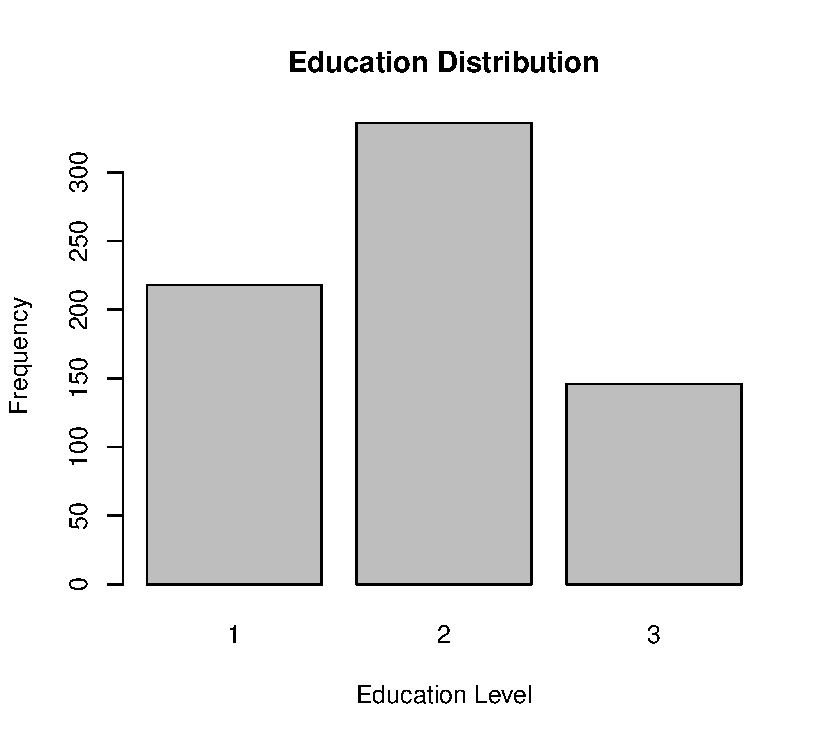
\includegraphics[width=\maxwidth]{Rplot2.pdf}
\caption{Bar plot of education}
\label{fig:2}
\end{figure}
\end{knitrout}


\noindent A plot of the histogram (Figure \ref{fig:2})shows that the most of the caregivers on average had attained Secondary school education.

\begin{knitrout}
\definecolor{shadecolor}{rgb}{0.969, 0.969, 0.969}\color{fgcolor}\begin{kframe}
\begin{alltt}
\hlcom{# Box plot of Income_Month by Depression Level}
\hlkwd{boxplot}\hlstd{(dataset}\hlopt{$}\hlstd{income_ksh} \hlopt{~} \hlstd{dataset}\hlopt{$}\hlstd{depression,} \hlkwc{main} \hlstd{=} \hlstr{"Income by Depression Level"}\hlstd{,} \hlkwc{xlab} \hlstd{=} \hlstr{"Depression Level"}\hlstd{,} \hlkwc{ylab} \hlstd{=} \hlstr{"Income"}\hlstd{)}
\end{alltt}
\end{kframe}
\begin{figure}[H]
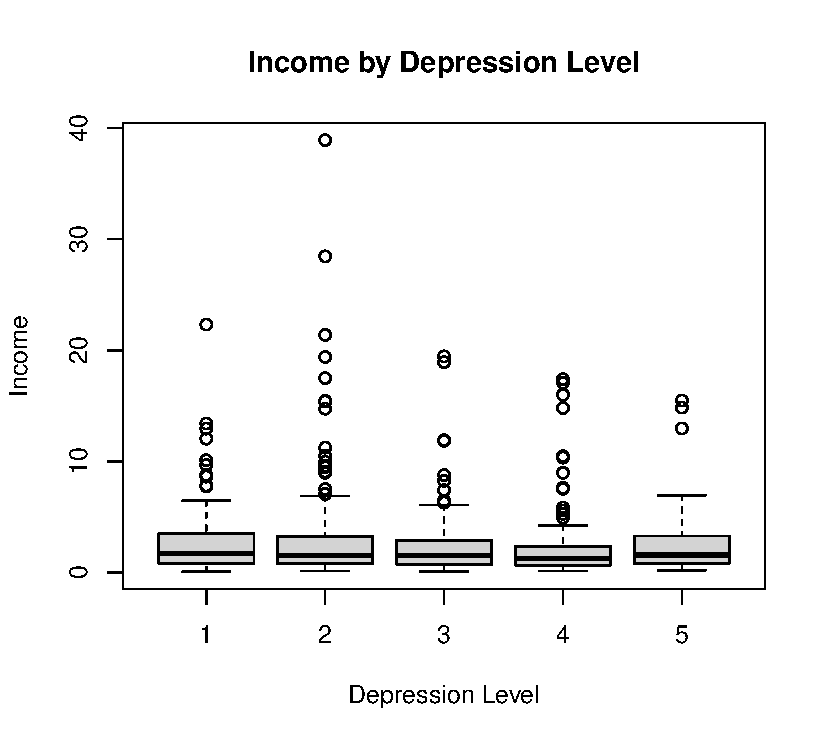
\includegraphics[width=\maxwidth]{Rplot3.pdf} 
\caption{Box plot of income by depression level}
\label{fig:3}
\end{figure}
\begin{kframe}\begin{alltt}
\hlcom{# Correlation matrix}
\hlkwd{names}\hlstd{(dataset)}
\end{alltt}
\begin{verbatim}
## [1] "age_participant" "age_patient"     "sex_participant" "sex_patient"    
## [5] "marital_status"  "education"       "income_ksh"      "social_support" 
## [9] "depression"
\end{verbatim}
\begin{alltt}
\hlstd{cor_matrix} \hlkwb{<-} \hlkwd{cor}\hlstd{(dataset[,} \hlkwd{c}\hlstd{(}\hlstr{"age_participant"}\hlstd{,} \hlstr{"age_patient"}\hlstd{,} \hlstr{"income_ksh"}\hlstd{)])}
\hlkwd{print}\hlstd{(cor_matrix)}
\end{alltt}
\begin{verbatim}
##                 age_participant age_patient  income_ksh
## age_participant      1.00000000  0.07172348 -0.04748347
## age_patient          0.07172348  1.00000000 -0.01814071
## income_ksh          -0.04748347 -0.01814071  1.00000000
\end{verbatim}
\end{kframe}
\end{knitrout}
\noindent The correlation matrix indicated a negative correlation between age of the care giver and the income the caregiver earns. It was noted that their is a negative correlation between age of the patient and income earned by the caregiver.

\begin{knitrout}
\definecolor{shadecolor}{rgb}{0.969, 0.969, 0.969}\color{fgcolor}\begin{kframe}
\begin{alltt}
\hlcom{# Pairwise scatter plot}
\hlkwd{pairs}\hlstd{(dataset[,} \hlkwd{c}\hlstd{(}\hlstr{"age_participant"}\hlstd{,} \hlstr{"age_patient"}\hlstd{,} \hlstr{"income_ksh"}\hlstd{)])}
\end{alltt}
\end{kframe}
\begin{figure}[H]
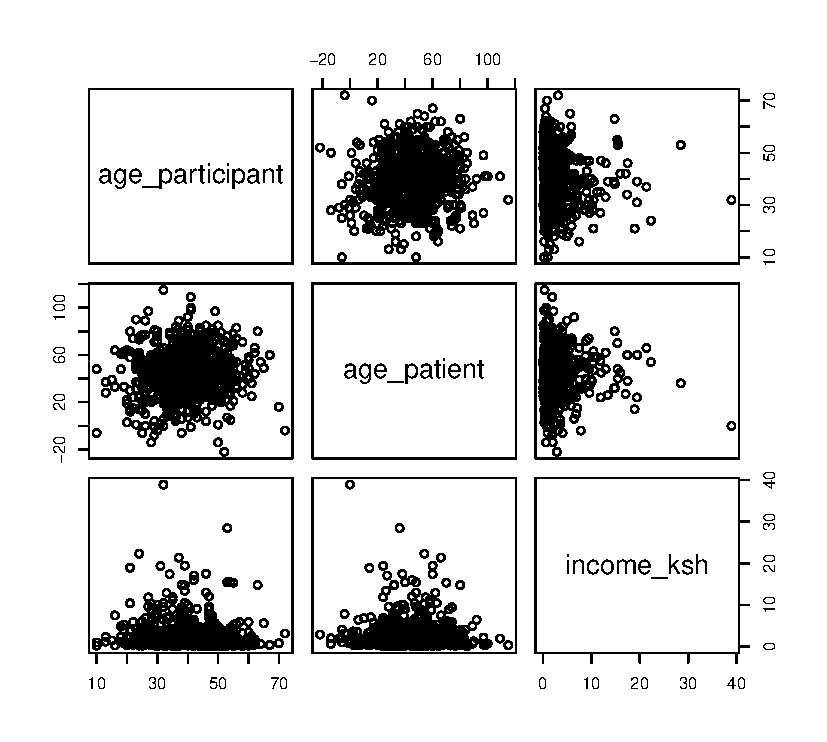
\includegraphics[width=\maxwidth]{Rplot4.pdf} 
\caption{Pairwise scatter plot}
\label{fig:4}
\end{figure}
\end{knitrout}


\noindent From Figure \ref{fig:4} the data forms ellipsoid clusters indicating that there is a relationship in the ages of the caregiver, age of patient and income of the caregiver.

\subsection{Ordinal Logistic Regression Model}
Below we used the \textbf{polr} command from the \textbf{MASS} package to estimate an Ordinal logistic regression model.
\begin{knitrout}
\definecolor{shadecolor}{rgb}{0.969, 0.969, 0.969}\color{fgcolor}\begin{kframe}
\begin{alltt}
\hlcom{# Fit an ordinal logistic regression model}
\hlstd{model} \hlkwb{<-} \hlkwd{polr}\hlstd{(depression} \hlopt{~} \hlstd{age_participant} \hlopt{+} \hlstd{age_patient} \hlopt{+}
                \hlstd{marital_status} \hlopt{+} \hlstd{education} \hlopt{+} \hlstd{income_ksh} \hlopt{+} \hlstd{social_support,}
              \hlkwc{data} \hlstd{= df,}\hlkwc{Hess}\hlstd{=}\hlnum{TRUE}\hlstd{)}
\end{alltt}
\end{kframe}
\end{knitrout}

\subsection{Data Interpretation and Discussions}
In this part, we interpret the results of our study and discussed their implications.
\begin{knitrout}
\definecolor{shadecolor}{rgb}{0.969, 0.969, 0.969}\color{fgcolor}\begin{kframe}
\begin{alltt}
\hlcom{# Print the model summary}
\hlcom{#model}
\hlkwd{summary}\hlstd{(model)}
\end{alltt}
\begin{verbatim}
## Call:
## polr(formula = depression ~ age_participant + age_patient + marital_status + 
##     education + income_ksh + social_support, data = df, Hess = TRUE)
## 
## Coefficients:
##                      Value Std. Error t value
## age_participant -0.0052639   0.006954  0.7569
## age_patient     -0.0008122   0.003406  0.2385
## marital_status   0.0758508   0.089496 -0.8475
## education        0.0496053   0.095367 -0.5201
## income_ksh       0.0133679   0.018344 -0.7287
## social_support  -0.0563137   0.149247  0.3773
## 
## Intercepts:
##     Value   Std. Error t value
## 1|2 -1.3819  0.3918    -3.5275
## 2|3  0.1779  0.3877     0.4589
## 3|4  1.2344  0.3906     3.1606
## 4|5  2.3874  0.4035     5.9168
## 
## Residual Deviance: 215.684 
## AIC: 235.684
\end{verbatim}
\end{kframe}
\end{knitrout}
\noindent  Let $X_1$= Age of caregiver, $x_2$= Age of the patient, $x_3$= marital status, $X_4$= Level of education, $x_5$= household income and $x_6$= social support, then our estimated model becomes;

$$logit(P(Y \leq 1)) = -1.38 - (-0.005)x_1 - (-0.0008)x_2 - (0.076)x_3 -(0.05)x_4 -(0.013)x_5 - (-0.056)x_6$$
$$	logit(P(Y \leq 2)) = 0.18 - (-0.005)x_1 - (-0.0008)x_2 - (0.076)x_3 -(0.05)x_4 -(0.013)x_5 - (-0.056)x_6$$
$$logit(P(Y \leq 3)) = 1.23-(-0.005)x_1 - (-0.0008)x_2 - (0.076)x_3 -(0.05)x_4 -(0.013)x_5 - (-0.056)x_6$$
$$logit(P(Y \leq 4)) = 2.39 - (-0.005)x_1 - (-0.0008)x_2 - (0.076)x_3 -(0.05)x_4 -(0.013)x_5 - (-0.056)x_6$$

\begin{knitrout}
\definecolor{shadecolor}{rgb}{0.969, 0.969, 0.969}\color{fgcolor}\begin{kframe}
\begin{alltt}
\hlcom{## store table}
\hlstd{(ctable} \hlkwb{<-} \hlkwd{coef}\hlstd{(}\hlkwd{summary}\hlstd{(model)))}
\end{alltt}
\begin{verbatim}
##                         Value  Std. Error    t value
## age_participant  0.0052639339 0.006954489  0.7569117
## age_patient      0.0008122355 0.003405856  0.2384821
## marital_status  -0.0758508009 0.089495806 -0.8475347
## education       -0.0496053286 0.095367414 -0.5201497
## income_ksh      -0.0133679199 0.018344140 -0.7287297
## social_support   0.0563137072 0.149247258  0.3773182
## 1|2             -1.3819499210 0.391768796 -3.5274630
## 2|3              0.1779383054 0.387722932  0.4589316
## 3|4              1.2344467404 0.390578115  3.1605630
## 4|5              2.3874338238 0.403501520  5.9167902
\end{verbatim}
\end{kframe}
\end{knitrout}

\noindent Next we see the estimates for the four intercepts. The intercepts indicate where the latent variable is cut to make the three groups that we observe in our data. \\~\\.


\begin{knitrout}
\definecolor{shadecolor}{rgb}{0.969, 0.969, 0.969}\color{fgcolor}\begin{kframe}
\begin{alltt}
\hlcom{## calculate and store p values}
\hlstd{p} \hlkwb{<-} \hlkwd{pnorm}\hlstd{(}\hlkwd{abs}\hlstd{(ctable[,} \hlstr{"t value"}\hlstd{]),} \hlkwc{lower.tail} \hlstd{=} \hlnum{FALSE}\hlstd{)} \hlopt{*} \hlnum{2}
\end{alltt}
\end{kframe}
\end{knitrout}
\noindent Finally, we see the residual deviance, -2 * Log Likelihood of the model as well as the AIC. Both the deviance and AIC are useful in model comparison.

\begin{knitrout}
\definecolor{shadecolor}{rgb}{0.969, 0.969, 0.969}\color{fgcolor}\begin{kframe}
\begin{alltt}
\hlcom{## combined table}
\hlstd{(ctable} \hlkwb{<-} \hlkwd{cbind}\hlstd{(ctable,} \hlstr{"p value"} \hlstd{= p))}
\end{alltt}
\begin{verbatim}
##                         Value  Std. Error    t value      p value
## age_participant  0.0052639339 0.006954489  0.7569117 4.491028e-03
## age_patient      0.0008122355 0.003405856  0.2384821 8.115072e-01
## marital_status  -0.0758508009 0.089495806 -0.8475347 3.966972e-03
## education       -0.0496053286 0.095367414 -0.5201497 6.029593e-03
## income_ksh      -0.0133679199 0.018344140 -0.7287297 4.661670e-03
## social_support   0.0563137072 0.149247258  0.3773182 7.059371e-03
## 1|2             -1.3819499210 0.391768796 -3.5274630 4.195624e-04
## 2|3              0.1779383054 0.387722932  0.4589316 6.462833e-03
## 3|4              1.2344467404 0.390578115  3.1605630 1.574645e-03
## 4|5              2.3874338238 0.403501520  5.9167902 3.282851e-09
\end{verbatim}
\end{kframe}
\end{knitrout}

\noindent For a unit increase in the age of a caregiver, the expected change of the value of depression in log odds scale is 0.005 given all the other variables are held constant.\\

\noindent For a unit increase in the age of the patient, the expected change of the value of depression in the log odds scale is 0.0008 given all the other variables are held constant.\\

\noindent For income, a one unit increase in income, we would expect a 0.013367 decrease in the expected value of depression in the log odds scale, given that all of the other variables in the model are held constant.\\

\noindent A unit increase in education(i.e from primary to secondary), we would expect a 0.05 decrease in the value of depression in the log odds scale, given that all of the other variables in the model are held constant.\\

 \noindent A one unit increase in marital status, we would expect a 0.076 decrease in the value of depression in the log odds scale, given that all of the other variables in the model are held constant.\\

\noindent A one unit increase in social support, the expected change in the value of depression in log odds scale is 0.06, given that all of the other variables in the model are held constant..\\

\subsection{Odds Ratio}
This subsection presents the odds ratios for our ordinal logistic regression model and discuss their implications of the odds ratios for  our model.
\begin{knitrout}
\definecolor{shadecolor}{rgb}{0.969, 0.969, 0.969}\color{fgcolor}\begin{kframe}
\begin{alltt}
\hlcom{## odds ratios}
\hlkwd{exp}\hlstd{(}\hlkwd{coef}\hlstd{(model))}
\end{alltt}
\begin{verbatim}
## age_participant     age_patient  marital_status       education      income_ksh 
##       1.0052778       1.0008126       0.9269545       0.9516049       0.9867210 
##  social_support 
##       1.0579295
\end{verbatim}
\begin{alltt}
\hlcom{## OR and CI}
\hlkwd{exp}\hlstd{(}\hlkwd{cbind}\hlstd{(}\hlkwc{OR} \hlstd{=} \hlkwd{coef}\hlstd{(model), ci))}
\end{alltt}
\begin{verbatim}
##                        OR     2.5 %   97.5 %
## age_participant 1.0052778 0.9916830 1.019104
## age_patient     1.0008126 0.9941470 1.007516
## marital_status  0.9269545 0.7776230 1.104571
## education       0.9516049 0.7892164 1.147162
## income_ksh      0.9867210 0.9516645 1.023043
## social_support  1.0579295 0.7894627 1.417498
\end{verbatim}
\end{kframe}
\end{knitrout}

\noindent We see that for the:
\begin{itemize}
\item \textbf{Age Caregiver:}\\
\noindent One unit increase in age of caregiver increases the odds of being depressed by 0.5\% assuming all other variables are held constant.

\item \textbf{Age Patient:}\\
\noindent One unit increase in age of the patient increases the odds of the caregiver being depressed by 0.08\% assuming all other variables are held constant.

\item \textbf{Marital Status:}\
\noindent Caregivers who are married (compared to those who are not) have lower odds of being in a higher depression level by approximately 8.4\%, assuming all other variables are held constant.
\item \textbf{Education:} \\
\noindent One-unit increase in Education(say from primary to secondary)reduces the odds of the caregive being depressed by 5.9\%,  assuming all other variables are held constant.

\item \textbf{Household Income:} \\
\noindent One-unit increase in Household income reduces the odds of being in higher depression level by 1.4\% assuming all other variables are held constant.

\item \textbf{Social\_Support:} \\
\noindent Caregivers involved in social support groups (compared to those not involved) have higher odds of being in a higher depression level by approximately 5.79\%, assuming all other variables are held constant.
\end{itemize}


\subsection{Likelihood Ratio Test}
\noindent The likelihood ratio test compares the fit of the fitted model with a null model that includes only the intercept. This helps determine whether the independent variables significantly improve the model fit. 
\begin{knitrout}
\definecolor{shadecolor}{rgb}{0.969, 0.969, 0.969}\color{fgcolor}\begin{kframe}
\begin{alltt}
\hlcom{# 1. Likelihood Ratio Test}
\hlstd{null_model} \hlkwb{<-} \hlkwd{polr}\hlstd{(depression} \hlopt{~} \hlnum{1}\hlstd{,} \hlkwc{data} \hlstd{= dataset)}
\hlcom{# Null model with only intercept}
\hlstd{likelihood_ratio} \hlkwb{<-} \hlkwd{anova}\hlstd{(null_model, model)}
\hlcom{# Likelihood ratio test}
\hlstd{likelihood_ratio}
\end{alltt}
\begin{verbatim}
## Likelihood ratio tests of ordinal regression models
## 
## Response: depression
##                                                                                      Model
## 1                                                                                        1
## 2 age_participant + age_patient + marital_status + education + income_ksh + social_support
##   Resid. df Resid. Dev   Test    Df LR stat.   Pr(Chi)
## 1       696   218.060                                
## 2       690   215.684 1 vs 2     6 2.375745 0.008821064
\end{verbatim}
\begin{alltt}
\hlstd{p_value_lr} \hlkwb{<-} \hlstd{likelihood_ratio}\hlopt{$}\hlstd{Pr[}\hlnum{2}\hlstd{]}
\hlcom{# p-value for the likelihood ratio test}
\hlstd{p_value_lr}
\end{alltt}
\begin{verbatim}
## [1] 0.008821064
\end{verbatim}
\end{kframe}
\end{knitrout}
\noindent The likelihood ratio test is significant suggesting that the independent variables collectively have a significant effect on the odds of being in a higher depression level.

\newpage

\section*{CHAPTER FIVE}
\section*{CONCLUSIONS}
	\addcontentsline{toc}{section}{5 CONCLUSIONS}
\setcounter{section}{5}
\setcounter{subsection}{0}
\subsection{Introduction}
This chapter presents the summary and the conclusions of the study in the subsections
that follow.
	\subsection{Summary}
In summary, significant depression predictors were identified, estimation and interpretation of coefficients of factors of depression were done and determination and interpretation of the odds ratios were done. 
\subsection{Conclusions}

In conclusion we found that the age of caregiver, Household income, level of education, Marital status of the caregiver and social support are significant in determining
the depression severity of cancer caregivers while the age of the patient was found
to be insignificant.
\newpage
\subsection{Recommendation}
Based on the findings of this research project, several evidence-based recommendations can be made to inform the development of targeted interventions for depression among cancer caregivers in rural settings:
\begin{enumerate}
	\item The Kenya National Bureau  of Statistics to conduct research and store data on Depression for future research.
	
	\item Given the role being performed by cancer caregivers, the government through state departments should develop intervetions to provide tailored support to cancer caregivers for better quality life of the patients. 
	
	\item Interventions should address the financial challenges faced by caregivers in rural areas, such as limited job opportunities or transportation costs. Offering financial assistance programs or connecting caregivers with available resources can help alleviate financial stress and improve their mental well-being.
\end{enumerate}
\newpage
\section*{REFERENCES}
	\addcontentsline{toc}{section}{REFERENCES}
\begin{enumerate}
	\item  Agresti A. (1996),  An Introduction to Categorical Data Analysis, New York: John Wiley \& Sons, Inc
	\item  Agresti A. (2002), Categorical Data Analysis, Second Edition, New Jersey: John Wiley \& Sons, Inc.
	\item Jain G., Roy A., Harikrishnan V., Yu S., Dabbous O. and Lawrence, C. (2013), Patient-Reported Depression Severity Measured by the PHQ-9 and Impact on Work Productivity, \emph{Journal of Occupational and Environmental Medicine}, 55(3), 252-258.
	\item Kaggwa M. M., Najjuka, S. M., Nuwamanya S., Nabulo, H., and Nkola R. (2021), Depression among cancer caregivers in a rural setting.xlsx.

	
	\item Laing S. S., and Jones S. M. (2016), Anxiety and Depression Mediate the Relationship between Perceived Workplace Health Support and Presenteeism, \emph{Journal of Occupational and Environmental Medicine}, 58(11), 1144-1149.
	
	\item Leung D. Y., Mak Y. W., Leung S. F., Chiang V. C. and Loke A. Y. (2020), Measurement Invariances of the PHQ‐9 Across Gender and Age Groups in Chinese Adolescents,\emph{ Asia‐Pacific Psychiatry}, 12(3).
	
	\item Levis B., Benedetti A. and Thombs B. D. (2019), Accuracy of Patient Health Questionnaire-9 (PHQ-9) For Screening to Detect Major Depression: Individual Participant Data Meta-Analysis,\emph{BMJ}.
	
	\item Levis B., Sun Y., He C., Wu Y., Krishnan A., Bhandari P. M. and Thombs B. D. (2020), Accuracy of the PHQ-2 Alone and in Combination with the PHQ-9 for Screening to Detect Major Depression: Systematic Review and Meta-Analysis,\emph{ JAMA}, 323(22), 2290-2300.
	
	\item Lister K., Seale J. and Douce C. (2023), Mental Health in Distance Learning: A Taxonomy of Barriers and Enablers to Student Mental Wellbeing, \emph{Open Learning: The Journal of Open, Distance and e-Learning}, 38(2), 102-116.
	
	
	\item Magtibay D. L., Chesak S. S., Coughlin K. and Sood, A. (2017), Decreasing Stress and Burnout in Nurses, \emph{The Journal of Nursing Administration}, 47(7/8), 391-395.
	
	\item Martin A., Sanderson K. and Cocker F. (2009), Meta-Analysis of the Effects of Health Promotion Intervention in the Workplace on Depression and Anxiety Symptoms,\emph{Scandinavian Journal of Work, Environment and Health}, 7-18.
	\item  Montgomery C. D, Peck A. E and Vining G.G.(2012), Introduction to linear regression analysis, John Wiley \& Sons Inc.
	\item Serpa J. G., Taylor S. L. and Tillisch K. (2014), Mindfulness-Based Stress Reduction (MBSR) Reduces Anxiety, Depression, and Suicidal Ideation in Veterans, \emph{Medical Care}, 52(12), S19-S24.
\end{enumerate}
\end{document}
